\chapter{Implementación}
En este capítulo se va a abordar la implementación del sistema. Para ello, en
primer lugar, se van a explicar las herramientas y tecnologías que se han utilizado
y el porqué de su elección. En segundo lugar, se explicará la implementación de la
base de datos, se mostrará el diagrama de clases y, por último, se explicará la
implementación de la aplicación, tanto del backend como del frontend.

\section{Herramientas y tecnologías}
En este apartado se van a explicar las herramientas y tecnologías utilizadas
para el desarrollo de la aplicación.

\subsection{Control de versiones}
Para realizar un seguimiento del desarrollo de la aplicación se ha utilizado la
herramienta de control de versiones \textit{Git} \cite{git}, que permite llevar un
control de los cambios realizados en el código fuente de la aplicación. Además, estos
cambios se han ido subiendo a la plataforma \textit{GitHub} \cite{github}.

Para seguir una estructura de los commits que se van realizando, se han ido escribiendo
los mensajes de commit con el formato "\texttt{<stack>} - \texttt{<mensaje>}", donde
\texttt{<stack>} es \textit{SERVER} o \textit{CLIENT} dependiendo de si el commit afecta
al backend o al frontend de la aplicación, y \texttt{<mensaje>} es la descripción de los
cambios que se han realizado.

En la figura \ref{fig:commits} se puede ver un ejemplo de una captura sacada
del listado de commits realizados en el repositorio de \textit{GitHub} \cite{github}.

\begin{figure}[H]
  \centering
  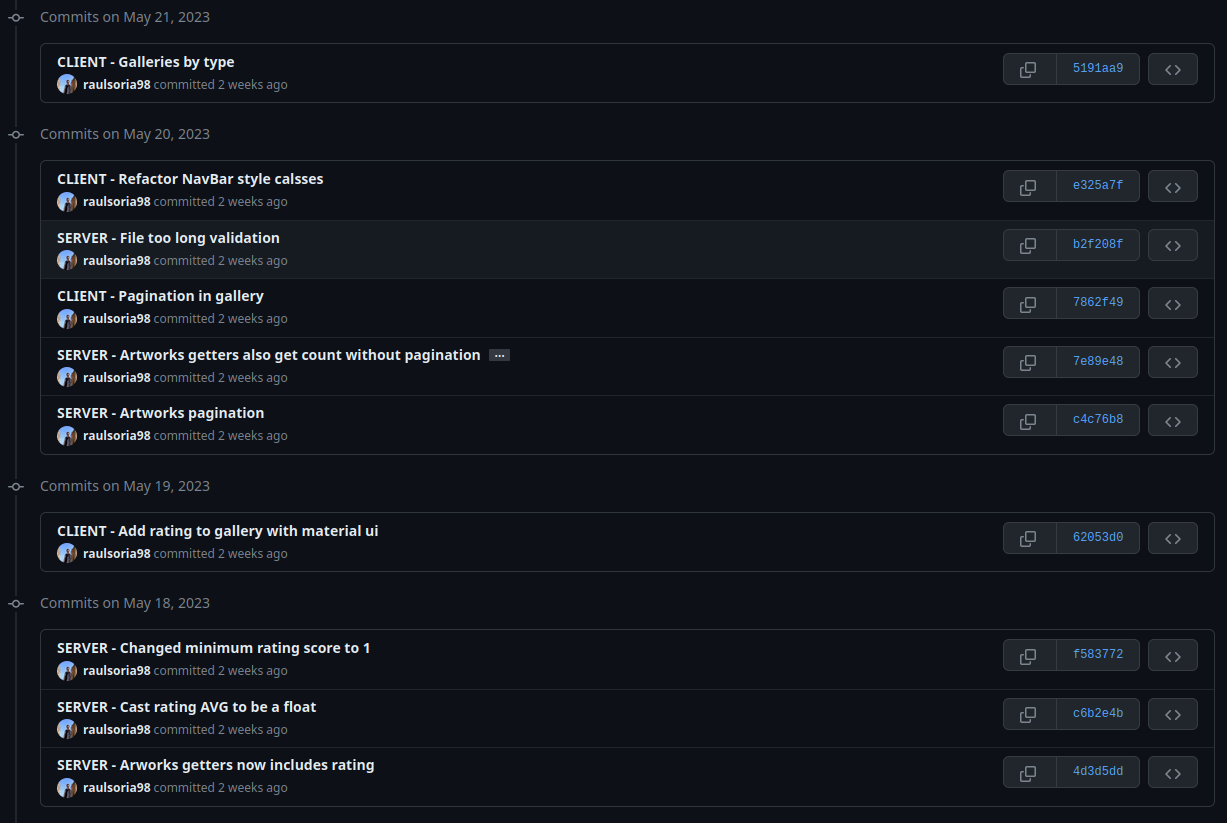
\includegraphics[width=1\textwidth]{commits}
  \caption{Ejemplo de mensajes de commit}
  \label{fig:commits}
\end{figure}

\subsection{Base de datos}
Para la base de datos había que elegir en primer lugar entre una base de datos
relacional o una base de datos no relacional.

En este artículo \cite{relational-vs-non-relational} se explica la diferencia entre
un tipo de base de datos y otro, las ventajas que tiene cada una y en qué casos es
más recomendable utilizar una u otra.

En el caso de nuestra aplicación, se ha optado por utilizar una base de datos relacional
ya que, aunque la base de datos no va a ser muy grande, sí que va a tener una estructura
bien definida con relaciones fuertes entre las tablas.

También es necesario elegir el gestor de base de datos que se va a utilizar, ya que
existen varios gestore de bases de datos relacionales. En nuestro caso se ha optado
por utilizar \textit{MySQL} \cite{mysql} ya que es el gestor de bases de datos
relacionales más utilizado y es el que más conozco personalmente.

\subsection{Backend}
Para el desarrollo del backend de la aplicación se ha utilizado \textit{Node.js}
\cite{nodejs} que es un entorno de ejecución de JavaScript. Se ha elegido este
entorno porque quería aprender a utilizarlo dada su popularidad y porque así podría
utilizar JavaScript tanto en el backend como en el frontend. Este último punto
hizo que descartara utilizar otros frameworks como \textit{Django} \cite{django}
o \textit{Ruby on Rails} \cite{ruby-on-rails}.

Como framework complementario a \textit{Node.js} se ha utilizado \textit{Express}
\cite{express} que facilita la creación de aplicaciones web y de APIs en \textit{Node.js}.

\subsection{Frontend}
Para el desarrollo del frontend de la aplicación se barajaron varias opciones.
En primer lugar, se pensó en utilizar \textit{Angular} \cite{angular} ya que es un
framework bastante popular y con el que ya había trabajado anteriormente. Sin embargo,
se descartó esta opción porque, como explican en este artículo \cite{angular-vs-react},
este es un framework muy completo y pensado para aplicaciones grandes donde prima el
trabajo en equipo ya que su estructura es fija y la esto la hace más compleja. Mientras
que \textit{React} \cite{react} es una librería más sencilla y flexible que permite
crear aplicaciones pequeñas como la nuestra de manera sencilla y sin una gran curva de
aprendizaje.

También se barajó la opción de utilizar \textit{Vue.js} \cite{vuejs} ya que es una
librería de la que también había oído hablar y que también usa JavaScript.
Como comentan en este otro artículo \cite{vuejs-vs-react}, \textit{Vue.js} \cite{vuejs}
también es una librería bastante sencilla y ligera, cuyos módulos se pueden ir añadiendo
según se vayan necesitando. Sin embargo, se descartó esta opción porque, aunque
\textit{Vue.js} \cite{vuejs} es más sencillo que \textit{React} \cite{react}, este
último tiene mayor rendimiento y me llamaba más la atención y quería aprender a
utilizarlo.


\section{Implementación de la base de datos}

\section{Diagrama de clases}

\section{Implementación de la aplicación}
